\section{Hardware}

\subsection{VR Headset}

\subsection{VR Controller}

\subsection{Tracker}

\subsection{Lichtboxen}\label{sec:lighthouse}

\subsection{Wireless Adapter }

\section{Software}

\subsection{Game Engine}

Es gibt mehrere Games Engines mit welchen eine VR Applikation geschrieben werden kann.
In Abbildung~\ref{fig:game_engine_marketshare} kann man den market share verschiedener Engines sehen.
Diese Daten sind aber mit vorsicht zu genießen, da das Skript welche diese Daten geliefert hat nach einigen Kriterien handelt.
Siehe~\cite{REDDIT_2018}.

\begin{figure}
    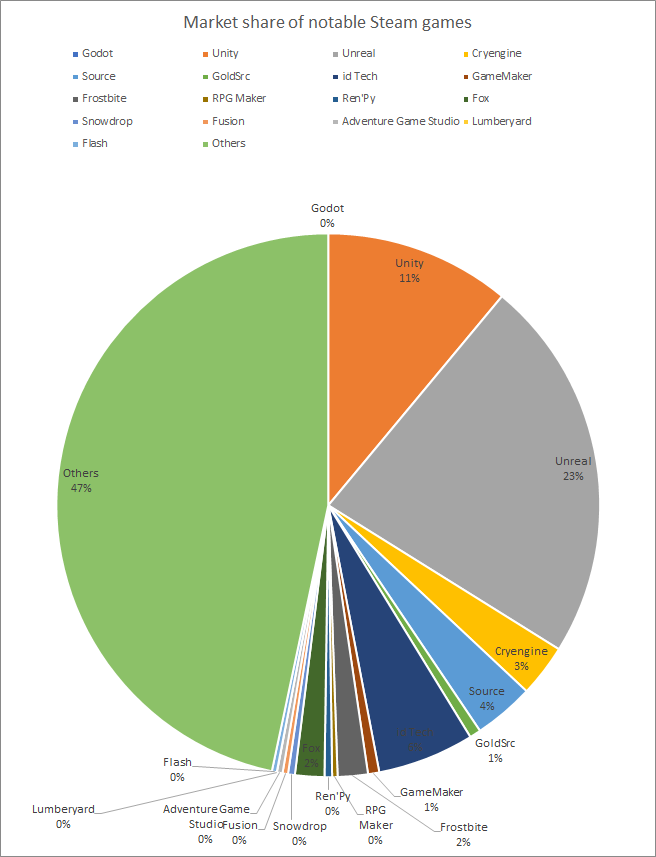
\includegraphics[scale=0.5]{pics/game_engine_marketshare}
    \caption{Game Engine Market-share}
    \label{fig:game_engine_marketshare}
\end{figure}

\subsubsection{Unity}

Unity ist eine Game Engine welche erstmals eine Apple exklusive Game Engine war und von Unity Technologies entwickelt worden ist.
Die Engine wurde weiter entwickelt und kann heute auch auf Windows und auf der Linux plattform benützt werden.
Die Engine ist gratis und wird von vielen als Einsteiger Engine beschrieben.
Auch sie eine Einsteiger Engine genannt wird heißt das nicht, dass sie in keinen professionellen Bereich benützt wird.
Viele bekannte Spiele wurden mit der Unity Engine entwickelt.
Im Besonderen sind viele Handyspiele mit dieser Engine entwickelt.
Spiele wie Pokemon GO, Among us und Hearthstone wurden in der Unity Engine entwickelt.

Vorteile:

\begin{itemize}
    \item Gratis Lizenz für persönlichen Nutzen und für Unternehmen mit unter 100000\$ Einkommen
    \item Programmierbar in der C# Programmiersprache
    \item Es kann fuer alle moeglichen Plattformen ein Programm geschrieben werden
    \begin{itemize}
        \item IOS
        \item Android
        \item Windows
        \item Linux
        \item usw.
    \end{itemize}
    \item verfügbaren Asset-store mit vielen verschiedenen fertigen Assets
\end{itemize}

Nachteile:

\begin{itemize}
    \item weniger Market-share~\ref{fig:game_engine_marketshare}
    \item geschlossener Source Code
\end{itemize}

\subsubsection{Unreal Engine}

Unreal Engine ist von Epic Games entwickelt.
Diese Engine ist eine weit verwendete Game Engine.
Dies kann man auch in Abbildung~\ref{fig:game_engine_marketshare} herausnehmen.
Unreal Engine findet ihren nutzen aber eher in der PC- und Konsolen-welt.
Viele Spiele wie Fortnite, Ark Survival Evolved, Borderlands 3 und Jedi Fallen Order sind mit dieser Engine entwickelt worden.

Vorteile:

\begin{itemize}
    \item großer Market-share~\ref{fig:game_engine_marketshare}
    \item "easy to learn" visual scripting
\end{itemize}

Nachteile

\begin{figure}
    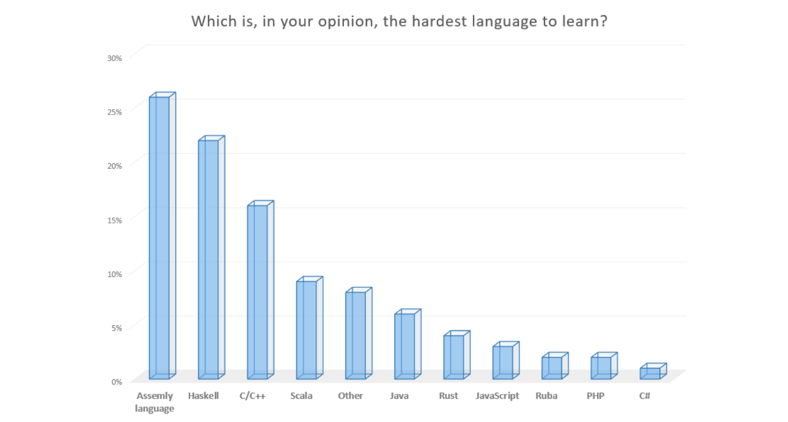
\includegraphics[scale=0.5]{pics/programming_languages_hardest}
    \caption{Schwerste Programmiersprachen}
    \label{fig:hardest_programming_languages}
\end{figure}

\begin{itemize}
    \item 5\% Nutzungshonorar, wenn das Einkommen eines Produktes über 1000000\$ ist
    \item für erweiterte funktionalität wird c++ welches nach Umfrage in der Abbildung~\ref{fig:hardest_programming_languages}~\cite{JAXCENTER_2018} die drittschwierigste Sprache ist
\end{itemize}

\subsection{VR Plugin}

\subsection{Steam}

\subsection{Vive Wireless}

\subsection{Final IK Plugin}

\subsection{IDE}

\subsection{Modellierung}
